% ---------------------------------------------------------------------------
% Payoff scale reshapes how language models play the prisoner's dilemma.
%
% Royal Society (Interface Focus) order: Introduction, Material and methods,
% Results, Discussion, Conclusion, back matter, numbered references.
%
%   pdflatex main && bibtex main && pdflatex main && pdflatex main
%
% Every number in this file is produced by Analysis/scaling/s00..s06 and the
% three tables are machine-generated into tables_auto.tex.  Do not retype them.
% s08_verify_paper.py re-checks every prose number against the data; run it
% after touching any figure quoted here.
% ---------------------------------------------------------------------------
% ---------------------------------------------------------------------------
% SUBMISSION ROUTE - READ BEFORE SUBMITTING.  % >>> FILL IN <<<
%
% Interface Focus does not accept unsolicited research articles.  It publishes
% theme issues only; every research article in the venue carries a publisher-
% inserted "One contribution of N to a theme issue '...'" footnote.  A
% manuscript uploaded without a commission is returned before review.  The two
% legitimate routes are (a) being named as an author in an accepted theme-issue
% proposal by a Guest Editor, or (b) proposing a theme issue to the publisher.
%
% If no invitation exists, retarget J. R. Soc. Interface (RSIF): same publisher,
% same house style, takes unsolicited research articles, overlapping scope.
% Everything below transfers unchanged.
%
% Record here which route applies:  [ ] Guest Editor invitation from ______
%                                   [ ] retargeted to RSIF
% ---------------------------------------------------------------------------
\documentclass[11pt,a4paper]{article}

\usepackage[T1]{fontenc}
\usepackage[utf8]{inputenc}
\usepackage{lmodern}
\usepackage[margin=1in]{geometry}
\usepackage{graphicx}
\usepackage{amsmath,amssymb}
\usepackage{booktabs}
\usepackage{caption}
\usepackage{authblk}
\usepackage[numbers,sort&compress]{natbib}
\usepackage{enumerate}       % \begin{enumerate}[(1)]: the numbered research
                             % questions in the Introduction
\usepackage{microtype}
\usepackage{url}\urlstyle{tt} % \path breaks long file paths at the slashes
\usepackage{xcolor}          % must precede hyperref: allcolors uses a mixed colour
\usepackage[colorlinks=true,allcolors=blue!55!black]{hyperref}
\setlength{\emergencystretch}{2em}

\captionsetup{font=small,labelfont=bf,width=\textwidth}
\setlength{\parskip}{0pt}
\renewcommand{\baselinestretch}{1.15}
\graphicspath{{figures/}}

\newcommand{\lam}{\lambda}
% The interval is always labelled: a bare bracketed pair is ambiguous between
% a confidence interval, a range and a support, and the venue never prints one.
\newcommand{\ci}[2]{(95\% CI #1, #2)}

\title{\bfseries Payoff scale reshapes how language models play the
prisoner's dilemma}

% ---------------------------------------------------------------------------
% >>> FILL IN <<<  AUTHOR LIST CARRIED OVER FROM THE COMPANION MANUSCRIPT.
%
% The author list below, its order, the equal-contribution daggers, the
% affiliations and the two corresponding authors were carried over from the
% companion manuscript by the same group, "Payoff scaling shapes cooperation in
% LLM agents across languages" (cited here as selfpreprint2026scaling), which
% reports the earlier and smaller collection on this project.  The present
% article reports a different corpus, so the list, the order and the
% equal-contribution marks MUST BE CONFIRMED FOR THIS PAPER BEFORE SUBMISSION:
% authorship follows the contribution to THIS work and not to the earlier one,
% and the CRediT statement in the back matter has to be written to match
% whatever list is confirmed here.
%
% ORCID is MANDATORY for the submitting author (it is entered in the submission
% system rather than printed by the journal) and strongly encouraged for the
% rest.  None is recorded in this repository and none has been invented here.
% Record them below before submission, one line per author:
%   ORCID  <submitting author>:  0000-0000-0000-0000   % >>> FILL IN <<<
%
% Use \texttt and not \path for the e-mail addresses: \path is fragile and
% \affil takes a moving argument.
% ---------------------------------------------------------------------------
\renewcommand\Authfont{\normalsize}
\renewcommand\Affilfont{\small}
\setlength{\affilsep}{0.7em}
\author[1,$\dagger$,$\ast$]{The Anh Han}
\author[2,4,$\dagger$]{Trung-Kiet Huynh}
\author[2,4,$\dagger$]{Dao-Sy Duy-Minh}
\author[3,4]{Thanh-Bang Cao}
\author[3,4]{Phong-Hao Le}
\author[3,4]{Hong-Dan Nguyen}
\author[2,4]{Phu-Quy Nguyen-Lam}
\author[3,4]{Minh-Luan Nguyen-Vo}
\author[3,4]{Hong-Phat Pham}
\author[2,4]{Phu-Hoa Pham}
\author[3,4]{Thien-Kim Than}
\author[3,4]{Chi-Nguyen Tran}
\author[3,4]{Huy Tran}
\author[3,4]{Gia-Thoai Tran-Le}
\author[5]{Alessio Buscemi}
\author[3,4,$\ast$]{Le Hong Trang}
\affil[1]{School of Computing, Engineering and Digital Technologies, Teesside
University, Middlesbrough, United Kingdom}
\affil[2]{Faculty of Information Technology, University of Science (HCMUS),
Ho Chi Minh City, Vietnam}
\affil[3]{Faculty of Computer Science and Engineering, Ho Chi Minh City
University of Technology (HCMUT), Ho Chi Minh City, Vietnam}
\affil[4]{Vietnam National University Ho Chi Minh City (VNU-HCM),
Ho Chi Minh City, Vietnam}
\affil[5]{Luxembourg Institute of Science and Technology (LIST), Luxembourg}
\affil[$\dagger$]{These authors contributed equally to this work.}
\affil[$\ast$]{Corresponding authors: Le Hong Trang,
\texttt{lhtrang@hcmut.edu.vn}; The Anh Han, \texttt{t.han@tees.ac.uk}}
\date{}

\begin{document}
\maketitle

% ---------------------------------------------------------------------------
% Abstract, subject areas and keywords.
%
% Word count of the abstract body: 199 words (Royal Society hard cap is 200).
% Counted with a whitespace split; "200,000" counts as one word.  ONE word of
% headroom - recount after every edit here, do not assume there is slack.
% One paragraph, no citations, no unexplained abbreviations or acronyms.
% Four numerals only: 200{,}000, 0.636, the confidence interval, and the
% "at most 1" threshold.
%
% Subject areas: carried over from the companion manuscript's \subject entry.
% Keywords: six, lower case, COMMA separated (the production style guide asks
% for commas and a maximum of six; the draft used semicolons).  Our preamble is
% article.cls plus authblk, which provides neither \subject nor \keywords, so
% both are set as bold run-in paragraphs.
% ---------------------------------------------------------------------------

\begin{abstract}
\noindent
Large language models are increasingly deployed as agents that negotiate and
decide for their users, so whether they cooperate is a governance question.
We ask how two everyday levers shape it: the size of what is at stake, and the
language the game is posed in. The first is unusual: multiplying every payoff by
a positive constant leaves preferences, best replies, equilibria and the orbits
of the replicator dynamics untouched, so its predicted behavioural effect is
zero by theorem, not convention. Using it as an instrument, five frontier
models played an iterated prisoner's dilemma across ten payoff scales, crossed
with prompt language and persona, on a balanced grid of 200{,}000 decisions.
Cooperation moves in every model, by up to 0.636 (95\% CI 0.588, 0.686),
differently in each, so averaging over models reports a movement no model makes.
Its size depends on the prompt language; the scale also gates the persona
instruction, reversing its sign in two models of five where every printed payoff
is at most 1. The effect is already present on the opening move, and what is
played changes too. Cooperation rates published for language models should be
read, and governed, alongside their sensitivity to payoff scale.
\end{abstract}

\noindent\textbf{Subject areas:} artificial intelligence, game theory,
multi-agent systems

\smallskip
\noindent\textbf{Keywords:} machine behaviour, large language models, iterated
prisoner's dilemma, payoff scaling, utility invariance, cross-lingual behaviour


% ---------------------------------------------------------------------------
% Section 1: Introduction.
%
% Restyled 2026-09-06 towards the register of the companion manuscript by the
% same group (dense citation, one paragraph per strand of literature, explicit
% numbered research questions, explicit numbered contributions).  Progression:
%   (i)    language models deployed as agents in cooperation dilemmas
%   (ii)   the game-theoretic evaluation literature and what it does not measure
%   (iii)  behavioural intention as a strategy, and its supervised inference
%   (iv)   cross-lingual non-invariance
%   (v)    prompt sensitivity more generally, and why none of it supplies a null
%   (vi)   the payoff rescaling, inert by theorem, then the gap paragraph
%   (vii)  machine behaviour, and what a scale-dependent rate does to it
%   (viii) four numbered research questions
%   (ix)   three numbered contributions
%   (x)    relation to the earlier collection by the present authors
%
% Numbers used here: "10{,}000 dyads" (research questions), and 0.636, 17.9%,
% 5.8%, 0.154 and 0.249 (contributions).  All already appear elsewhere in the
% manuscript and are checked by Analysis/scaling/s08_verify_paper.py.  Counts of
% models, languages, scales, questions and contributions are design facts, not
% statistics.
% ---------------------------------------------------------------------------

\section{Introduction}
\label{sec:intro}

Large language models are increasingly deployed as \emph{agents} that negotiate,
coordinate and decide on behalf of their users, in recommendation systems,
negotiation tools and multi-agent
assistants~\citep{park2023generative,tessler2024ai,hammond2025multi,cook2024llm}.
In these settings behaviour emerges from strategic interaction rather than from
isolated model outputs, and the agents meet \emph{cooperation dilemmas} whose
resolution bears directly on safety, coordination and AI
governance~\citep{dafoe2021cooperative,lu2024llms,han2026social,idowu2026mapping}.
A fast-growing literature measures how they behave when they do, with the
instruments of behavioural economics and cognitive
psychology~\citep{binz2023using,horton2023large,aher2023using} and with the
classical games~\citep{mei2024turing}. Equally consequential is how far that
behaviour adapts to the costs and benefits at issue, since a deployed agent
meets the same dilemma at many different magnitudes~\citep{hammond2025multi}.

A growing body of work evaluates language models through game-theoretic lenses,
and in particular through matrix and repeated games, reporting systematic
departures from equilibrium play, persistent cooperative biases and sensitivity
to contextual factors such as language and
incentives~\citep{fairgame2025,sun2025gtllm_survey,mao2025alympics,pal2026strategiescooperationdefectionlarge,willis2025will,fan2024can,pires2025large,fu2026optimal}.
The prisoner's dilemma is the workhorse of that literature, its strategy space
mapped and its predictions
sharp~\citep{axelrod1981evolution,axelrod1984evolution,nowak1992tit,nowak1993strategy,nowak2006five,press2012iterated}.
Within it the models turn out to be individual rather than uniform, differing in
how readily they retaliate~\citep{akata2023playing}, how readily they
forgive~\citep{fontana2024nicer}, how much weight they give the game rather than
the story around it~\citep{lore2024strategic} and how far an instructed
disposition carries into conditioned
reciprocity~\citep{phelps2023investigating}. These studies share two unremarked
reporting conventions. Each summarizes a model by a cooperation rate, or a few
of them, measured at one payoff matrix; and each reports what the agents did
rather than the decision rule that produced it.

Evaluating strategic behaviour at the level that alignment and governance
require therefore asks for more than aggregate outcomes. Drawing on behavioural
and evolutionary game theory~\citep{sigmund:2010bo}, a behavioural intention can
be conceptualised as an agent's \emph{strategy}: a decision rule mapping an
interaction history to the next
action~\citep{han2011role,diStefanoIntention2023,Han2012ALIFEjournal,fujimoto2019functional}.
The canonical strategies of repeated games, Always Cooperate, Always Defect,
Tit-for-Tat and Win-Stay-Lose-Shift~\citep{Axelrod1980Effective,sigmund:2010bo},
supply an interpretable vocabulary for such intentions, and prior work has shown
that they can be inferred from noisy behavioural trajectories by supervised
learning~\citep{han2011role,diStefanoIntention2023} and extended by
probabilistic models to mixed or stochastic play~\citep{inferenceStrategies}.
The inference is not free. Separating the memory-one rules from observed play
has been shown to need a long run of observations even where the resident rule
is fixed by construction~\citep{kim2021win}, which is why the read-out used here
is reported as a resemblance, with its provenance beside it
(\S\ref{sec:readout}).

In parallel, what a language model does is not invariant across the language it
is addressed in~\citep{fairgame2025}. Strategic reasoning, risk sensitivity and
cooperation patterns depend on linguistic framing, sometimes by margins
comparable to the differences between
models~\citep{lore2024strategic,buscemi2025llms,buscemi2025strategic}. Whether
the strategies agents play are themselves language-dependent, and whether that
dependence introduces systematic bias into multi-agent settings, is largely
open.

That dependence is one instance of a wider pattern: what is measured on a
language model depends on things the measurement was not about. Accuracy moves
with the order of the in-context examples~\citep{lu2022fantastically}, and with
formatting choices that leave the meaning of the prompt intact, by margins wide
enough to swamp the differences between the models being
compared~\citep{sclar2024quantifying}. Instructions about who the model is are
equally consequential: a persona changes what a model
produces~\citep{deshpande2023toxicity}, shifts measured
capability~\citep{salewski2023context} and, conditioned on a demographic
backstory, reproduces the response distribution of the matching human
subgroup~\citep{argyle2023out}. What none of these manipulations can supply is a
null.

The choice of units is not usually stated as a design decision at all, because
in the theory it is not one. A payoff matrix is a von Neumann--Morgenstern
utility, defined only up to a positive affine
transformation~\citep{vonneumann1944theory,luce1957games}, so writing the same
dilemma with cells ten times larger changes no preference, no best reply, no
equilibrium and no orbit of the replicator dynamics. Under the theory the two
matrices are not two games written differently. They are one game. The theory of
the iterated dilemma inherits the indifference, turning on the ordering of the
four payoffs and on ratios among them and never on their absolute
size~\citep{axelrod1981evolution,nowak1992tit,nowak1993strategy,press2012iterated},
and the modelling literature normalizes the scale
away~\citep{szabo2007evolutionary,perc2010coevolutionary}. Current theory works
at the indifference rather than merely permitting it: where social learners
update on the payoff they last received, the condition for conditional
cooperation to persist under strong selection loses the benefit and the cost of
cooperation altogether and turns on the ordering of the payoffs
alone~\citep{glynatsi2024evolution}.

The invariance belongs to the theory, not to people: human valuation is neither
linear in magnitude nor anchored at zero~\citep{kahneman1979prospect}, and human
choice reverses between logically equivalent descriptions of one
problem~\citep{tversky1981framing}. That gap has been argued to be structural
rather than incidental, with the linguistic description of an action entering
the utility function directly and a shift proposed from outcome-based to
language-based preferences~\citep{capraro2024language}.

Two things are established, and they have not been put together. The first is
that what a language model does depends on features of the prompt that carry
no task content: the order of the examples, the formatting, the persona, the
language. The second is that multiplying every payoff by a positive constant
carries no task content in the strictest sense available, because the matrix
it produces is not a second game but the same one. What is not known is
whether the strategic behaviour of a language model respects that invariance.
To our knowledge, no study has asked. Every manipulation in the sensitivity
literature could legitimately change behaviour, so a measured change under any
of them is at worst a nuisance and at best a finding, against an expected
effect nobody had specified. The same holds of the human framing results that
motivate language-based preferences, where a label such as donate rather than
boost carries connotation, so what is under test there is an assumption about
preferences and not a theorem about their
representation~\citep{capraro2024language}. A rescaling is the one manipulation
whose expected effect is specified, and specified as zero, so a measured
departure has a stated reference value rather than a comparison condition.

What follows if the invariance fails is a question about what a published
cooperation rate means. Machine behaviour proposes that autonomous systems be
studied empirically, with the instruments of the behavioural sciences, because
what such a system does is not deducible from how it was
built~\citep{rahwan2019machine}. Those instruments arrive with a known
difficulty: a behavioural manipulation almost never carries a predicted effect,
so a measured change has to be read against a comparison condition the
experimenter chose. The invariance classes of decision theory are the exception,
supplying a manipulation whose predicted effect is a stated number, and the
number is zero.

The consequences run through the strands of machine behaviour this study
touches. The persona line is the one place where the experimenter addresses the
agent about its social role, and whether it takes hold turns out to depend on
the units the matrix was printed in. The departure is already present on the
opening move, which locates it in the reading of the matrix rather than in the
weighing of a history. We report no evolutionary dynamics of our own; what we
report is a constraint on an input such dynamics take, since models of mixed
human-machine populations carry the cooperativeness of the artificial agent as a
parameter and ask where the population
settles~\citep{santos2018social,han2011intention,han2013good,perc2017statistical,paiva2018engineering}.
A rate partly determined by the experimenter's units is not the quantity those
models need, and if the dependence takes a different form in each model it is
invisible to exactly the pooled designs the field uses to summarize many models
at once.

Together, these considerations let us put four questions to the rescaling:
\begin{enumerate}[(1)]
\item Does strategic behaviour survive multiplying every payoff by a positive
      constant, and by how much does it fail to?
\item Does the answer depend on the prompt language, and on the persona the
      model is told to adopt?
\item Does the rescaling change only how often a model cooperates, or also the
      strategy it is playing?
\item Does the effect enter at the opening move, or through the course of play?
\end{enumerate}
We answer them on a complete and exactly balanced grid of 10{,}000 dyads
(\S\ref{sec:methods}).

Here, we turn a theorem into an instrument. The contributions of the present
paper are: \textbf{(i)} a payoff-rescaling protocol whose predicted behavioural
effect is exactly zero, used to ask whether five frontier language models are
playing the game they were shown (\S\ref{sec:game}); all five depart from the
invariance, by up to 0.636 in cooperation. \textbf{(ii)} a per-model analysis
showing that the departure has a different shape in each model, to the point of
anticorrelation, so that what a pooled analysis reports is a movement no model
in the pool makes: the interaction of the payoff scale with the model carries
$17.9\%$ of the variance across cells against $5.8\%$ for the main effect, and
averaging the five curves gives a range of 0.154 where the mean within-model
range is 0.249. The main effect is significant here only because one model
departs far enough to survive the averaging, which is a fact about that model
rather than a property of language models in general, and a panel assembled
without it returns no significant main effect at all. The same holds one level
down, since the size of the departure depends on the prompt language as well as
on the model, so that per-model, per-language reporting is a matter of validity
rather than of presentation. \textbf{(iii)} evidence that the departure is
structural and not a shift in level: the payoff scale gates the persona
instruction, reversing its sign in two models of five and abolishing it in a
third, play becomes measurably less consistent with any canonical memory-one
rule in four models of five while the fifth shows no trend, and the effect is
already present on the opening move, before any history exists.

An earlier and smaller collection on this project has been reported separately
by the present authors~\citep{selfpreprint2026scaling}: three models at three
payoff scales, in the same five prompt languages, with cooperation read off the
trajectories and reported as rising with the stakes. The present article differs
in what it collects and in what it claims. It collects six models rather than
three and ten payoff scales rather than three, spanning five orders of
magnitude, on a grid whose completeness and balance are enforced by the analysis
build rather than assumed. It frames the rescaling as an invariance whose
predicted effect is a theorem rather than as a manipulation of the stakes whose
effect was expected. And it reports every quantity per model, which is what
shows the movement to be heterogeneous, with one of the five running downwards,
and the pooled statement to be an artefact of averaging.

% NOTE TO AUTHORS.  The scope-and-limitations paragraph that used to close this
% section has been folded into \S4.5, where the venue puts limitations; nothing
% it said is lost.
%
% NOTE TO AUTHORS.  Royal Society practice expects prior related work by the
% same authors to have its relationship to the present article stated.  That
% relationship is now stated in the closing paragraph above, against
% selfpreprint2026scaling, which is also cited in Methods for the polarity
% check.  The description of the earlier collection is drawn from the companion
% manuscript itself and should be checked against its final version before
% submission.  % >>> FILL IN <<<


% ---------------------------------------------------------------------------
% Section 2: Material and methods.
%
% Restructured 2026-09-06 to the shape of the companion manuscript:
%   2.1 Framework                        (FAIRGAME, what we extended, the grid)
%   2.2 The payoff-scaled prisoner's dilemma
%                                        (matrix, framing, ordering, the ten
%                                         lambdas, the invariance statement,
%                                         then models, languages, personas and
%                                         the collection protocol)
%   2.3 Strategy read-out
%   2.4 Statistical analysis             (fourth subsection: the specification
%                                         does not fit the companion's three)
%
% Nothing from the previous six subsections has been dropped.  The old
% "Experimental design" is now the second half of 2.1; the old "Models, prompt
% languages and personas" and "Protocol and data collection" are the second
% half of 2.2, which is where the companion puts the same material; the old
% "Statistical analysis" is 2.4 unchanged in substance.
%
% NOTES FOR THE AUTHORS - two corrections against an older draft, both
% following the code rather than the prose:
%   (1) a model-by-language-by-scale cell holds 40 dyads, not 200; 200 is the
%       size of a model-by-scale cell.  An older Methods said 250 cells of 200
%       dyads, which multiplies out to 50,000 rather than 10,000.
%   (2) the achieved parse-failure and fallback rates are not carried in the
%       released tables, so only the 0.02 assertion threshold is stated.
% ---------------------------------------------------------------------------

\section{Material and methods}
\label{sec:methods}

\subsection{Framework}
\label{sec:framework}

This study runs the protocol of FAIRGAME, the Framework for AI Agents Bias
Recognition using Game Theory~\citep{fairgame2025}, which supports systematic and
reproducible evaluation of language models through controlled game-theoretic
experiments: an experimental condition fixes the payoff structure, the horizon,
the model backend and the prompt language, and the repeated normal-form game is
then simulated and logged round by round. We did not run the reference
implementation. The models studied here are served through a benchmarking
platform the reference implementation does not address, so the protocol was
reimplemented against that platform, reproducing FAIRGAME's language-specific
prompt templates byte for byte, its reply parsing and its penalty scoring, and
writing the same per-game table schema. The templates are compared against the
reference files before every collection run, because one save in the wrong
encoding corrupts the prompt that reaches the model rather than a comment beside
it. Three things are ours rather than the protocol's. First, the payoff-scaling
factor applied to the prisoner's dilemma, which is the manipulation this paper is
about (\S\ref{sec:game}). Second, a completeness guard that refuses to release an
analysis table unless the grid is exactly balanced and internally consistent.
Third, a strategy read-out that reports which canonical memory-one rule a
trajectory most resembles, and with what provenance (\S\ref{sec:readout}).

The design is a complete factorial crossing of six language models, ten payoff
scales, five prompt languages, four persona pairings and ten replicates.

The unit of collection is the dyad, one ten-round game between two agents of the
same model, contributing two agent-games, an agent-game being the ten decisions
one agent takes in one game. Each of the 300
model-by-language-by-scale cells holds exactly 40 dyads, the four persona
pairings by ten replicates; pooling the five languages gives 200 dyads and 400
agent-games in each of the 60 model-by-scale cells. The corpus is 12{,}000
dyads, 24{,}000 agent-games and 240{,}000 decisions.

Five of the six models are reported in the main text and the sixth, Gemini 3.1
Flash-Lite, in the electronic supplementary material, for the reason given with
the models below. The five carry 250 of the cells, 10{,}000 dyads, 20{,}000
agent-games and 200{,}000 decisions, and are the grid every main-text figure and
table is computed on. Balance is enforced rather than assumed: the build refuses
to write its tables unless every cell is complete and each game's recorded
payoffs recover the scale its cell was run at (electronic supplementary
material, \S S1).

\subsection{The payoff-scaled prisoner's dilemma}
\label{sec:game}

Both agents receive the prisoner's-dilemma prompt of the FAIRGAME
protocol~\citep{fairgame2025} in its no-communication, announced-horizon
condition. It casts the game as a criminal interrogation, states the four
payoffs as penalties, names the two actions OptionA and OptionB,
carries the running history of play, announces the ten-round horizon and
instructs the agent to minimize its penalty.

At $\lam = 1$ the agent is shown $T = 0$, $R = 2$, $P = 6$, $S = 10$ in penalty
units, in the usual temptation, reward, punishment and sucker notation. The
ordering $T < R < P < S$ is the image of the familiar $T > R > P > S$ on
utilities
$u = -\text{penalty}$, and $2R > T + S$ holds on those utilities, so alternation
is not preferred to mutual cooperation. OptionA pays less in both
columns and is therefore the dominant, defecting action, while mutual OptionB at
2 beats mutual OptionA at 6 and is the cooperative one; cooperation means
OptionB throughout this paper. The polarity was checked against the data as well
as against the prompt~\citep{selfpreprint2026scaling} (electronic supplementary
material, \S S1).

The manipulation multiplies all four cells by a positive constant $\lam$
(figure~\ref{fig:scaling}a), taking ten values spanning five orders of
magnitude, $\lam \in \{0.01, 0.1, 0.25, 0.5, 1, 2, 5, 10, 100, 1000\}$, and
changes nothing else in the prompt (electronic supplementary material, \S S2).
Two details bear on interpretation: $T = 0$ prints as 0 at every scale, so only
three of the four numbers move, and the history block records realised
penalties, so $\lam$ is present in every prompt of the game and not only the
first. We treat the printed penalties as the agent's utilities, as the prompt's
minimization instruction directs; because $\lam u$ with $\lam > 0$ is a positive
affine transformation of a von Neumann--Morgenstern
utility~\citep{vonneumann1944theory,luce1957games}, the predicted effect on an
agent playing the game is exactly zero. It is this that separates the present
manipulation from a manipulation of the stakes, whose behavioural effect is
expected rather than specified~\citep{kahneman1979prospect,tversky1981framing}.
An agent that instead applies a
non-linear valuation to the printed penalties is not bound by the invariance;
\S\ref{sec:discussion} returns to readings of that kind.

Six frontier models were run, each against itself; two different models were
never paired. They were Claude Haiku 4.5, GPT-5.4 Nano, Gemini 3.5 Flash-Lite,
Qwen3 235B-A22B, Grok 4.20 and Gemini 3.1 Flash-Lite, served through the Kaggle
Benchmarks model proxy on an OpenAI-compatible chat-completions endpoint. Their
endpoint identifiers, four dated and two not, are in the electronic
supplementary material, \S S2.

The main text reports the first five of them. The sixth, Gemini 3.1 Flash-Lite,
is reported in full in the electronic supplementary material, \S S8, and the
reason is a property of its endpoint rather than of its results: its identifier
names an endpoint that is both undated and announced as provisional, so what was
served under that name while the corpus was collected cannot be re-addressed
afterwards. We state the cost of drawing the line there rather than leaving it
to be found. \path{gemini-3.5-flash-lite}, which stays in the main text, is an
undated alias as well and could in principle be re-pointed to a later build, so
its results carry a weaker form of the same risk; the line drawn here is between
an identifier marked provisional and one that is not, and not between pinned and
unpinned. It is also the one model of the six whose strategy trend
runs opposite to the rest (\S\ref{sec:results}), which is a reason to report it
prominently rather than to set it aside. Every quantity the main text gives for
the five is given for all six in the electronic supplementary material, which
also states what including it changes, and on every conclusion of this paper
that is nothing.
% >>> FILL IN <<<  State the collection date range for these six endpoints in
% the electronic supplementary material.  For hosted proprietary models served
% from an unpinned endpoint, the date is the only thing that fixes what was
% actually run, and it is not recorded anywhere in this repository.

The prompt languages are English, French, Vietnamese, Chinese and Arabic, in
templates byte-identical to the FAIRGAME resource files and checked against them
before every collection run (electronic supplementary material, \S S2).
Artefacts of those files are reproduced rather than repaired, the consequential
one being that the Arabic and Chinese versions state the four cells as penalties
but phrase the goal sentence as maximizing a reward, so we treat the five
languages as five distinct stimuli rather than five renderings of one.

Each agent also receives one line naming its persona, in the language of the
prompt: in English, \emph{You are cooperative.} or \emph{You are selfish.} The
two are crossed in all four ordered pairings, ten replicates each. The
opponent's persona is never disclosed (electronic supplementary material,
\S S2), so a pairing reaches a player only through realised behaviour and not
before round 2, and we treat it as a design factor and a regression covariate
rather than as information the agent held.

Every game runs ten rounds with simultaneous moves: both agents see the same
history, rounds 1 to $r-1$, and the round is scored once both have replied.
Sampling runs at temperature 1.0, under a common-random-numbers scheme that
gives a given round of a given replicate the same seed at every payoff scale
(electronic supplementary material, \S S2.1).

Decisions are elicited as free text and parsed by the protocol's own matcher. A
reply it cannot resolve is regenerated, up to two further attempts, and if all
three fail the decision is recorded as OptionA, which under this framing is
defection: the fallback can only push a measured cooperation rate down, never
up, and it cannot manufacture the cooperative behaviour reported here. Each
collection run asserts that its fallback rate is at most 0.02, but the achieved
rates are not carried in the released per-game tables, so we cannot report how
they vary with the payoff scale (electronic supplementary material, \S S2.2).

\subsection{Strategy read-out}
\label{sec:readout}

The read-out reports which of four canonical rules, AllC, AllD, Tit-for-Tat and
Win-Stay-Lose-Shift, a ten-round trajectory most \emph{resembles}. It is not an
identification of the strategy a model is running, and no claim in this paper
treats it as one.

All four rules are memory-one, so exact matching is a lookup with no learning in
it, and it returns a \emph{set} rather than a label, because over ten rounds
several rules routinely prescribe the same moves. The three provenances, the
agent-games matched exactly by one rule (deduced), by several at once
(ambiguous) and by none (unmatched), are recorded separately and never merged,
and the same matcher yields a continuous quantity needing no labels at all, the
number of rounds violating the nearest rule.

Where the rules leave the answer open a single-layer
LSTM~\citep{hochreiter1997long} arbitrates. Trained on the synthetic corpus
alone, which contains no language-model output, it reaches $98.5\%$ accuracy in
distribution and $93.6\%$ and $81.1\%$ on two execution-noise levels held out
entirely (electronic supplementary material, \S S6). It ranks only within the
set the rule base returns, so it can never overturn a deduction; it decides
alone only where no rule fits, and its share of the labels is very unevenly
spread across the four rules, which bounds how the composition may be read
(\S\ref{sec:results}).

\subsection{Statistical analysis}
\label{sec:stats}

The cooperation rate of an agent-game is the share of its ten decisions that are
OptionB; a cell mean averages the agent-games of a cell, and round-level
analyses use the binary decision itself. Because the two agents of a dyad play
each other and the ten rounds inside an agent-game are strongly autocorrelated,
every interval was computed by resampling whole dyads with replacement,
1{,}500 draws, percentile method~\citep{efron1993introduction}, and every
regression clustered its standard errors on the dyad (electronic supplementary
material, \S S2.3).
Because the range over the ten scales is a maximum minus a minimum, and so
positive by construction, its bootstrap interval quantifies the precision of the
range and not its distance from zero; the permutation test supplies the test.

Because the null is a theorem, the matching test destroys the association with
the payoff scale and leaves the rest of the design as observed: the scale label
is shuffled among whole dyads, the unit to which the scale was assigned, and the
range of the ten scale means recomputed (electronic supplementary material,
\S S2.3).

For each model we fitted a logistic regression of the round-level decision on
the payoff scale as a ten-level factor, with prompt language, own persona and
opponent persona as covariates, $\lam = 1$ as reference and standard errors
clustered on the dyad, and tested the nine scale contrasts jointly by a Wald
test (table~\ref{tab:effect}). The variance decomposition is a type-II analysis
of variance on the 250 cell means of the five models reported here, with terms
for model, language and payoff scale and their three two-way interactions and no
three-way term, so the residual on 144 degrees of freedom is the omitted
three-way interaction; the same decomposition on all 300 cells is in the
electronic supplementary material, \S S4.

Every payoff printed is at most 1 exactly when $\lam \leq 0.1$, which two of the
ten scales satisfy. The persona result contrasts those two scales with the
remaining eight, as a difference of differences with an interval from the same
dyad bootstrap; where a trend across the whole grid is wanted instead,
$\log_{10}\lam$ enters as a continuous predictor. Analyses were run in Python,
and the package versions are listed in the electronic supplementary material,
\S S9.


% ---------------------------------------------------------------------------
% Section 3, Results.  Six subsections merged into four.
%
% Old 2.1 (Design) is deleted: Materials and methods now precedes Results and
% carries the design, the guard on cell completeness and the action mapping.
% Old 2.2 + 2.3 -> 3.1 ; old 2.4 + 2.5 -> 3.2 ; old 2.6 -> 3.3 ; old 2.7 -> 3.4.
%
% Every numeral below is carried verbatim from the previous draft, from
% tables_auto.tex or from supplementary.tex.  Nothing is recomputed or
% re-rounded here.  Two numbers that lived only in the Discussion, the
% corpus-wide provenance split and its two label-level deduced shares, have
% been moved into 3.3; see the report accompanying this fragment.
%
% All six figure environments and % Generated by Analysis/scaling/s06_tables.py - do not edit by hand.
\begin{table}[t]
\centering
\caption{\textbf{Cooperation over the ten payoff scales, by model.}
Minimum, maximum and range, with a 95\% confidence interval on the range from a
bootstrap over whole dyads and a permutation test on the payoff-scale label
($0.0005$ is the floor of 2{,}000 draws). The last two columns test the nine
scale contrasts jointly in a per-model logistic regression of the round-level
decision, clustered on the dyad. Each entry pools 200 dyads per scale; ranges
are computed before rounding. Full specification in the electronic
supplementary material.}
\label{tab:effect}
\small
\begin{tabular}{lccccccc}
\toprule
& \multicolumn{2}{c}{cooperation} & & & & \multicolumn{2}{c}{Wald test} \\
\cmidrule(lr){2-3} \cmidrule(lr){7-8}
Model & min & max & range & 95\% CI & $p_{\text{perm}}$ & $\chi^2_9$ & $p$ \\
\midrule
Claude Haiku 4.5 & 0.371 & 0.452 & 0.081 & [0.062,\,0.135] & $0.0025$ & 32.3 & $<0.001$ \\
GPT-5.4 Nano & 0.438 & 0.680 & 0.243 & [0.200,\,0.290] & $0.0005$ & 164.1 & $<0.001$ \\
Gemini 3.5 Flash-Lite & 0.682 & 0.872 & 0.190 & [0.165,\,0.240] & $0.0005$ & 129.0 & $<0.001$ \\
Qwen3 235B-A22B & 0.399 & 0.494 & 0.095 & [0.068,\,0.158] & $0.0005$ & 96.9 & $<0.001$ \\
Grok 4.20 & 0.274 & 0.910 & 0.636 & [0.588,\,0.686] & $0.0005$ & 1227.3 & $<0.001$ \\
\bottomrule
\end{tabular}
\end{table}

\begin{table}[t]
\centering
\caption{\textbf{Persona effect below and above the sub-unit boundary, by
model.} Cooperation under a cooperative persona minus cooperation under a
selfish one, at the two scales where every printed payoff is at most 1
($\lam \leq 0.1$) and at the eight where some payoff exceeds it. Intervals are
95\% confidence intervals from the dyad bootstrap. A sign flip needs both
regime intervals to exclude zero on opposite sides, so a supra-unit interval
straddling zero means the effect is abolished rather than reversed.}
\label{tab:persona}
\footnotesize
\setlength{\tabcolsep}{3pt}
\begin{tabular}{lccccc}
\toprule
& \multicolumn{2}{c}{persona effect, with 95\% CI} & & & \\
\cmidrule(lr){2-3}
Model & $\lam \leq 0.1$ & $\lam \geq 0.25$ & shift & 95\% CI & sign flip \\
\midrule
Claude Haiku 4.5 & $-0.222$ $[-0.258,\,-0.186]$ & $+0.207$ $[+0.189,\,+0.226]$ & 0.429 & [0.389,\,0.471] & yes \\
GPT-5.4 Nano & $-0.135$ $[-0.179,\,-0.091]$ & $+0.018$ $[-0.001,\,+0.037]$ & 0.153 & [0.105,\,0.200] & no \\
Gemini 3.5 Flash-Lite & $-0.456$ $[-0.507,\,-0.406]$ & $+0.224$ $[+0.207,\,+0.242]$ & 0.680 & [0.625,\,0.736] & yes \\
Qwen3 235B-A22B & $-0.911$ $[-0.931,\,-0.893]$ & $-0.679$ $[-0.694,\,-0.664]$ & 0.233 & [0.210,\,0.258] & no \\
Grok 4.20 & $-0.441$ $[-0.485,\,-0.396]$ & $-0.303$ $[-0.326,\,-0.279]$ & 0.138 & [0.090,\,0.185] & no \\
\bottomrule
\end{tabular}
\end{table}

\begin{table}[t]
\centering
\caption{\textbf{Rule agreement and rule distance against the payoff scale,
by model.} Left, the share of agent-games matched exactly by one canonical
rule, below and above the sub-unit boundary, with the coefficient of a logistic
regression of that indicator on $\log_{10}\lam$; right, the mean number of
rounds violating the nearest canonical rule at the smallest and largest scale,
with the same trend by least squares. Both $\beta$ are per decade of $\lam$ and
their signs differ between models. Both cluster on the dyad, and neither block
uses the learned classifier.}
\label{tab:strategy}
\small
\setlength{\tabcolsep}{4pt}
\begin{tabular}{lcccccccc}
\toprule
& \multicolumn{4}{c}{exactly one rule fits (\%)}
& \multicolumn{4}{c}{rounds violating the nearest rule} \\
\cmidrule(lr){2-5} \cmidrule(lr){6-9}
Model & $\lam \leq 0.1$ & $\lam \geq 0.25$ & $\beta$ & $p$
      & $\lam{=}0.01$ & $\lam{=}10^3$ & $\beta$ & $p$ \\
\midrule
Claude Haiku 4.5 & 17.9 & 3.5 & $-0.545$ & $<0.001$ & 1.70 & 2.02 & $+0.073$ & $<0.001$ \\
GPT-5.4 Nano & 9.8 & 7.6 & $-0.038$ & $0.441$ & 2.02 & 2.19 & $+0.038$ & $0.052$ \\
Gemini 3.5 Flash-Lite & 32.2 & 15.6 & $-0.242$ & $<0.001$ & 0.48 & 1.36 & $+0.194$ & $<0.001$ \\
Qwen3 235B-A22B & 72.1 & 53.6 & $-0.267$ & $<0.001$ & 0.27 & 1.14 & $+0.202$ & $<0.001$ \\
Grok 4.20 & 44.6 & 17.1 & $-0.301$ & $<0.001$ & 0.92 & 0.37 & $-0.118$ & $<0.001$ \\
\bottomrule
\end{tabular}
\end{table}
 are preserved, in the
% float order of the previous draft.
% ---------------------------------------------------------------------------

\section{Results}
\label{sec:results}

Across the 240{,}000 recorded decisions of the whole corpus, the sixth model
included, cooperation is 0.5895; the five models reported below carry 200{,}000
of those decisions.

\subsection{Cooperation moves under a transformation that cannot matter}

Cooperation depends on the payoff scale in all five models
(figure~\ref{fig:scaling}b, table~\ref{tab:effect}). The range across the ten
scales runs from 0.081 \ci{0.062}{0.135} in Claude Haiku 4.5 to 0.636
\ci{0.588}{0.686} in Grok 4.20.

The observed range falls in the extreme upper tail of the permuted distribution
in every model ($p = 0.0005$ in four of the five, the smallest value 2{,}000
draws can return, and $p = 0.0025$ in Claude Haiku 4.5), and the per-model
logistic regression rejects the joint null on the nine scale contrasts
($\chi^2_9 = 32.3$ to $1227.3$, all $p \leq 2\times10^{-4}$), the largest
contrast against $\lam = 1$ ranging from 0.36 to 3.74 in log-odds
(table~\ref{tab:effect}).

The shapes are unlike one another. Grok 4.20 cooperates 0.274 at $\lam = 0.01$,
the lowest rate these data contain, and 0.910 at $\lam = 2$, the highest: the
same model, shown the same game, is predominantly a defector at the bottom of
the grid and predominantly a cooperator at the top. The others move less, and
disagree with it and with each other. GPT-5.4 Nano rises steeply from 0.438 at
$\lam = 0.01$ and saturates near 0.65; Claude Haiku 4.5 dips to a minimum at
$\lam = 0.25$ and recovers; Gemini 3.5 Flash-Lite oscillates within a high band;
Qwen3 235B-A22B drifts downward across the whole range.

\begin{figure}[t]
\centering
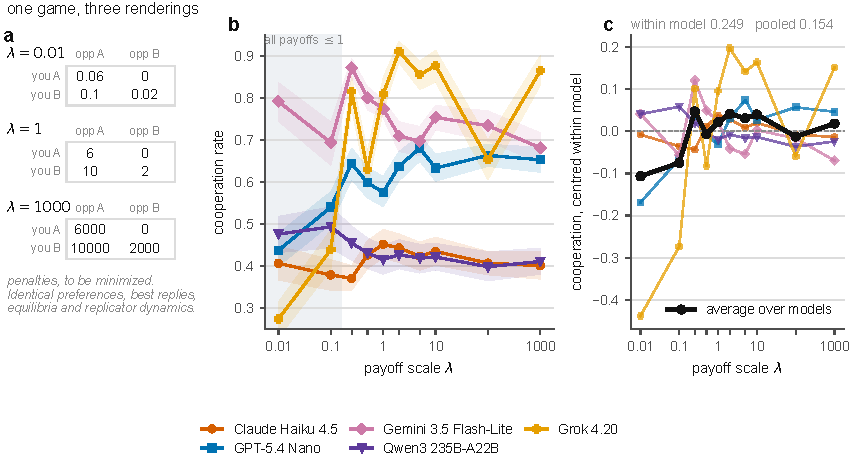
\includegraphics[width=\textwidth]{fig1_scaling.pdf}
\caption{\textbf{Cooperation against the payoff scale in five language models.}
(a) The same prisoner's dilemma at three payoff scales, shown to the agent as
penalties to be minimized.
(b) Cooperation against the payoff scale, one curve per model; the shaded band
marks the two scales at which every payoff printed is at most 1.
(c) The curves of (b) centred within model, with their average in black. Each
point in (b) and (c) averages 200 dyads, with 95\% percentile intervals from
1{,}500 bootstrap resamples of whole dyads.}
\label{fig:scaling}
\end{figure}

% Generated by Analysis/scaling/s06_tables.py - do not edit by hand.
\begin{table}[t]
\centering
\caption{\textbf{Cooperation over the ten payoff scales, by model.}
Minimum, maximum and range, with a 95\% confidence interval on the range from a
bootstrap over whole dyads and a permutation test on the payoff-scale label
($0.0005$ is the floor of 2{,}000 draws). The last two columns test the nine
scale contrasts jointly in a per-model logistic regression of the round-level
decision, clustered on the dyad. Each entry pools 200 dyads per scale; ranges
are computed before rounding. Full specification in the electronic
supplementary material.}
\label{tab:effect}
\small
\begin{tabular}{lccccccc}
\toprule
& \multicolumn{2}{c}{cooperation} & & & & \multicolumn{2}{c}{Wald test} \\
\cmidrule(lr){2-3} \cmidrule(lr){7-8}
Model & min & max & range & 95\% CI & $p_{\text{perm}}$ & $\chi^2_9$ & $p$ \\
\midrule
Claude Haiku 4.5 & 0.371 & 0.452 & 0.081 & [0.062,\,0.135] & $0.0025$ & 32.3 & $<0.001$ \\
GPT-5.4 Nano & 0.438 & 0.680 & 0.243 & [0.200,\,0.290] & $0.0005$ & 164.1 & $<0.001$ \\
Gemini 3.5 Flash-Lite & 0.682 & 0.872 & 0.190 & [0.165,\,0.240] & $0.0005$ & 129.0 & $<0.001$ \\
Qwen3 235B-A22B & 0.399 & 0.494 & 0.095 & [0.068,\,0.158] & $0.0005$ & 96.9 & $<0.001$ \\
Grok 4.20 & 0.274 & 0.910 & 0.636 & [0.588,\,0.686] & $0.0005$ & 1227.3 & $<0.001$ \\
\bottomrule
\end{tabular}
\end{table}

\begin{table}[t]
\centering
\caption{\textbf{Persona effect below and above the sub-unit boundary, by
model.} Cooperation under a cooperative persona minus cooperation under a
selfish one, at the two scales where every printed payoff is at most 1
($\lam \leq 0.1$) and at the eight where some payoff exceeds it. Intervals are
95\% confidence intervals from the dyad bootstrap. A sign flip needs both
regime intervals to exclude zero on opposite sides, so a supra-unit interval
straddling zero means the effect is abolished rather than reversed.}
\label{tab:persona}
\footnotesize
\setlength{\tabcolsep}{3pt}
\begin{tabular}{lccccc}
\toprule
& \multicolumn{2}{c}{persona effect, with 95\% CI} & & & \\
\cmidrule(lr){2-3}
Model & $\lam \leq 0.1$ & $\lam \geq 0.25$ & shift & 95\% CI & sign flip \\
\midrule
Claude Haiku 4.5 & $-0.222$ $[-0.258,\,-0.186]$ & $+0.207$ $[+0.189,\,+0.226]$ & 0.429 & [0.389,\,0.471] & yes \\
GPT-5.4 Nano & $-0.135$ $[-0.179,\,-0.091]$ & $+0.018$ $[-0.001,\,+0.037]$ & 0.153 & [0.105,\,0.200] & no \\
Gemini 3.5 Flash-Lite & $-0.456$ $[-0.507,\,-0.406]$ & $+0.224$ $[+0.207,\,+0.242]$ & 0.680 & [0.625,\,0.736] & yes \\
Qwen3 235B-A22B & $-0.911$ $[-0.931,\,-0.893]$ & $-0.679$ $[-0.694,\,-0.664]$ & 0.233 & [0.210,\,0.258] & no \\
Grok 4.20 & $-0.441$ $[-0.485,\,-0.396]$ & $-0.303$ $[-0.326,\,-0.279]$ & 0.138 & [0.090,\,0.185] & no \\
\bottomrule
\end{tabular}
\end{table}

\begin{table}[t]
\centering
\caption{\textbf{Rule agreement and rule distance against the payoff scale,
by model.} Left, the share of agent-games matched exactly by one canonical
rule, below and above the sub-unit boundary, with the coefficient of a logistic
regression of that indicator on $\log_{10}\lam$; right, the mean number of
rounds violating the nearest canonical rule at the smallest and largest scale,
with the same trend by least squares. Both $\beta$ are per decade of $\lam$ and
their signs differ between models. Both cluster on the dyad, and neither block
uses the learned classifier.}
\label{tab:strategy}
\small
\setlength{\tabcolsep}{4pt}
\begin{tabular}{lcccccccc}
\toprule
& \multicolumn{4}{c}{exactly one rule fits (\%)}
& \multicolumn{4}{c}{rounds violating the nearest rule} \\
\cmidrule(lr){2-5} \cmidrule(lr){6-9}
Model & $\lam \leq 0.1$ & $\lam \geq 0.25$ & $\beta$ & $p$
      & $\lam{=}0.01$ & $\lam{=}10^3$ & $\beta$ & $p$ \\
\midrule
Claude Haiku 4.5 & 17.9 & 3.5 & $-0.545$ & $<0.001$ & 1.70 & 2.02 & $+0.073$ & $<0.001$ \\
GPT-5.4 Nano & 9.8 & 7.6 & $-0.038$ & $0.441$ & 2.02 & 2.19 & $+0.038$ & $0.052$ \\
Gemini 3.5 Flash-Lite & 32.2 & 15.6 & $-0.242$ & $<0.001$ & 0.48 & 1.36 & $+0.194$ & $<0.001$ \\
Qwen3 235B-A22B & 72.1 & 53.6 & $-0.267$ & $<0.001$ & 0.27 & 1.14 & $+0.202$ & $<0.001$ \\
Grok 4.20 & 44.6 & 17.1 & $-0.301$ & $<0.001$ & 0.92 & 0.37 & $-0.118$ & $<0.001$ \\
\bottomrule
\end{tabular}
\end{table}


That disagreement has a direct consequence for reporting. Averaging the five
model curves gives a pooled curve whose range is
0.154, while the mean within-model range is 0.249, an attenuation of $1.62$
times (figure~\ref{fig:scaling}c). The pairwise correlations between model curves
average $-0.10$ and run from $-0.72$ to $+0.85$, with six of the ten pairs
negative. Curves that move in opposite directions cancel when added.

A variance decomposition on the 250 cell means makes the same point in another
currency. The model
accounts for $45.4\%$ of the
variance across cells and the model-by-language interaction for $17.0\%$. The
payoff scale carries $5.8\%$ as a main effect and is significant
($F_{9,144} = 10.64$, $p < 10^{-3}$), but its interaction with the model
carries $17.9\%$, three times as much ($p < 10^{-3}$), so most of what the
payoff scale does is specific to the model rather than shared across models.
Its interaction with the prompt language carries $3.6\%$ ($p = 0.018$), the
weakest test reported here.

That the main effect is significant at all is a fact about one model rather than
about language models. It is carried by Grok 4.20, whose departure is large
enough to survive being averaged with four others; a panel assembled without
that model returns no significant main effect, with every remaining model still
moving. A pooled analysis therefore reports a quantity whose significance turns
on which models happen to be in the panel, and whose size, 0.154 against a
typical within-model 0.249, matches no member of it.

\subsection{The size of the scale effect depends on the prompt language}

Neither prompt factor outside the game is neutral with respect to the payoff
scale. Both the level of cooperation and its sensitivity to the scale differ
with the prompt language (figure~\ref{fig:language}). Level differences are
large and model-specific, which is why the model-by-language interaction
dominates the decomposition above: Claude Haiku 4.5 cooperates 0.574 in Chinese
and 0.234 in Vietnamese, while GPT-5.4 Nano cooperates 0.798 in English and
0.458 in Arabic.

One caveat attaches to the level comparison rather than to the scale result.
The Arabic and Chinese templates, reproduced unaltered from the protocol, state
the four cells as penalties while phrasing the goal sentence as maximizing a
reward (\S\ref{sec:methods}), so a level difference between two languages here
is a difference between two stimuli and not between two renderings of one. It
cannot produce a dependence on the payoff scale, because the wording is
identical at every scale, and the ranges below are computed within a language.

The sensitivity differences are the new observation. The range of cooperation
across the ten scales itself depends on the language: 0.130 in Vietnamese
against 0.314 in French for Claude Haiku 4.5, and 0.162 in Chinese against 0.412 in
English for Gemini 3.5 Flash-Lite. Across the 25 model-language pairs it runs
from 0.083, in Qwen3 235B-A22B in French, to 0.855, in Grok 4.20 in English.
Scale sensitivity is a property of the model and the language together, not of
the model alone.

\begin{figure}[t]
\centering
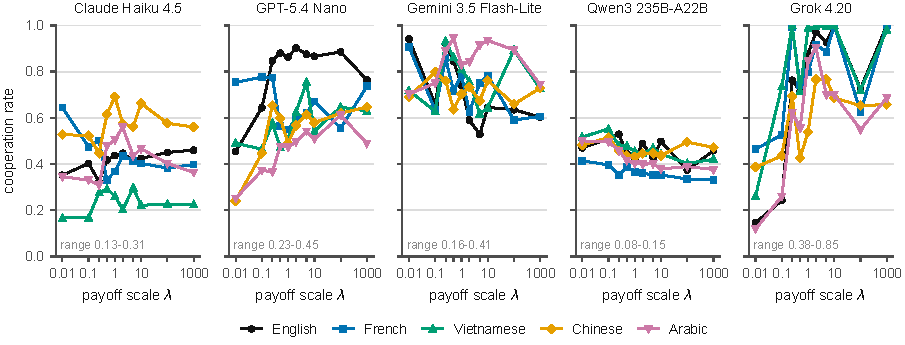
\includegraphics[width=\textwidth]{fig2_language.pdf}
\caption{\textbf{Cooperation against the payoff scale, by model and prompt
language.} One panel per model, one curve per prompt language; the annotation
gives the smallest and largest across-scale range among that model's five
languages. Each point averages 40 dyads.}
\label{fig:language}
\end{figure}

\subsection{The payoff scale gates the persona instruction}

The difference between the cooperation rates of the two persona instructions
measures how much the persona takes hold. It depends on the payoff scale, and
not gradually (figure~\ref{fig:persona}, table~\ref{tab:persona}). The natural
boundary is where the printed numbers stop being sub-unit, at $\lam \leq 0.1$
(\S\ref{sec:methods}). The persona effect shifts across it in all five models
and every shift excludes zero, from 0.138 \ci{0.090}{0.185} in Grok 4.20 to
0.680 \ci{0.625}{0.736} in Gemini 3.5 Flash-Lite.

Whether the sign reverses is the stronger claim, and we hold it to a test on
each regime rather than to a comparison of two point estimates. Two models of
five reverse: in Gemini 3.5 Flash-Lite and Claude Haiku 4.5 the sub-unit
interval lies wholly below zero and the supra-unit interval wholly above it, so
below the boundary these models cooperate \emph{more} when told they are
selfish. In GPT-5.4 Nano the supra-unit interval straddles zero, so its effect
is abolished at the boundary rather than reversed, and the other two models keep
their sign throughout.

The boundary appears to be one of magnitude rather than of decimal notation. At
$\lam = 0.25$ the payoffs are $0, 0.5, 1.5, 2.5$: still decimals, but no longer
all below 1, and there the persona effect already has its supra-unit sign and
size in both reversing models. The grid does not cross notation with magnitude
fully, since every sub-unit scale in it is decimal-printed too.

Qwen3 235B-A22B and Grok 4.20 invert the persona instruction at every scale
rather than only below the boundary (table~\ref{tab:persona}), apparently
resolving the story's ambiguity about who one cooperates with, one's partner or
the authorities, opposite to the convention the payoff matrix encodes. The
inversion is not our subject, but its magnitude depends on the payoff scale like
everything else measured here (electronic supplementary material, \S S5).
% The two regime means (-0.911, -0.679) and the two persona-level cooperation
% rates (0.072, 0.798) are printed in Table 2 and in ESM S5 respectively; the
% per-scale sequence is not monotone, so no trend is asserted here.

\begin{figure}[t]
\centering
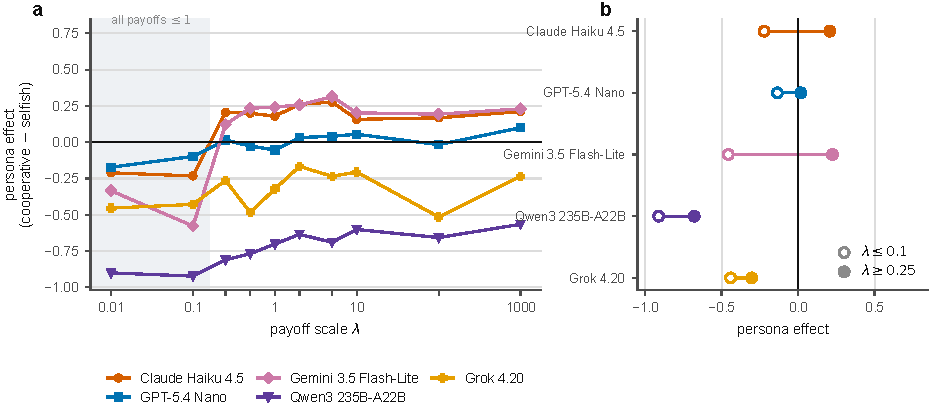
\includegraphics[width=\textwidth]{fig3_persona.pdf}
\caption{\textbf{The persona effect against the payoff scale.} The persona
effect is the cooperation rate under a cooperative persona minus that under a
selfish one.
(a) The effect against the payoff scale, each point averaging 200 dyads; the
shaded band marks the two scales at which every payoff printed is at most 1.
(b) The same contrast as two regime means: open markers at $\lam \leq 0.1$,
filled markers at $\lam \geq 0.25$ (table~\ref{tab:persona}).}
\label{fig:persona}
\end{figure}

\subsection{The scale also changes what is played}

Two models with the same cooperation rate can be
playing different games, so we read each agent-game against the four canonical
memory-one strategies (\S\ref{sec:methods}). What the read-out returns is a
resemblance and not an identification, and the labels below should be read that
way throughout. Over the whole corpus, all six models included, $23.0\%$ of
agent-games are matched
exactly by one rule, $17.5\%$ by several at once and $59.6\%$ by none.
% The corpus-wide split 23.0 / 17.5 / 59.6 previously appeared in main.tex only
% in the Discussion.  It is moved here, where the three provenances are named,
% because the Discussion is being stripped of statistics.

Play becomes less rule-governed as the payoffs grow in four models of five, and
shows no trend in the fifth (figure~\ref{fig:strategy}a,
table~\ref{tab:strategy}). Pooling the five, the share matched exactly by one
canonical rule falls from $38.6\%$ at $\lam = 0.01$ to $17.3\%$ at
$\lam = 10^{3}$, and the share matched by none rises from $51.6\%$ to $64.0\%$.
The trend is significant and negative in Claude Haiku 4.5 ($\beta = -0.545$ per
decade of $\lam$), Grok 4.20 ($-0.301$), Qwen3 235B-A22B ($-0.267$) and Gemini
3.5 Flash-Lite ($-0.242$), and absent in GPT-5.4 Nano ($p = 0.44$).

No model in the main text runs the other way on this measure, and one model in
the corpus does, so the claim should not be read as uniform. The sixth model,
Gemini 3.1 Flash-Lite, which is reported in the electronic supplementary
material because its identifier names an unpinned preview endpoint rather than
because of anything in its results (\S\ref{sec:methods}), carries a significant
positive trend ($\beta = +0.125$), its play becoming \emph{more} consistent with
a canonical rule as the payoffs grow. It is the only model of the six that does.
Over the whole corpus the result is therefore four models moving one way, one
showing no trend and one moving the other, and that is the form the evidence
supports.

The continuous version needs no labels at all: the number of rounds violating
the nearest canonical rule (figure~\ref{fig:strategy}b). It rises from 0.48 to
1.36 in Gemini 3.5 Flash-Lite and from 0.27 to 1.14 in Qwen3 235B-A22B between
the smallest and largest scale, with significant positive trends there and in
Claude Haiku 4.5. Grok 4.20 moves the other way, falling from 0.92 to 0.37
($\beta = -0.118$, $p < 0.001$): within the main five, three drift away from the
canonical rules as the payoffs grow and one drifts towards them.

The composition shifts too, and the models do not shift together
(figure~\ref{fig:mix}). Pooled across the five, the AllC share rises from
$38.1\%$ to $45.8\%$ of agent-games between the extreme scales and the
Tit-for-Tat share from $9.1\%$ to $12.7\%$, both at the expense of AllD, which
falls from $43.6\%$ to $28.3\%$. That pooled figure conceals the same
cancellation: GPT-5.4 Nano moves from $29.8\%$ to $50.7\%$ AllC while its AllD
share falls from $46.0\%$ to $17.5\%$, whereas Gemini 3.5 Flash-Lite moves the
other way on AllC, from $73.8\%$ to $51.5\%$, with Tit-for-Tat roughly doubling
from $6.8\%$ to $14.2\%$.

This last result leans hardest on the learned component, and the provenance is
not uniform across the four labels: AllC and AllD are anchored in part by exact
matching, whereas $94.6\%$ and $97.1\%$ of the Tit-for-Tat and
Win-Stay-Lose-Shift labels are attributions made where no canonical rule fits
(electronic supplementary material, \S S6.2). A movement in the Tit-for-Tat
share is therefore a statement about which canonical rule the play most
resembles, not a claim that the model is running Tit-for-Tat.

\begin{figure}[t]
\centering
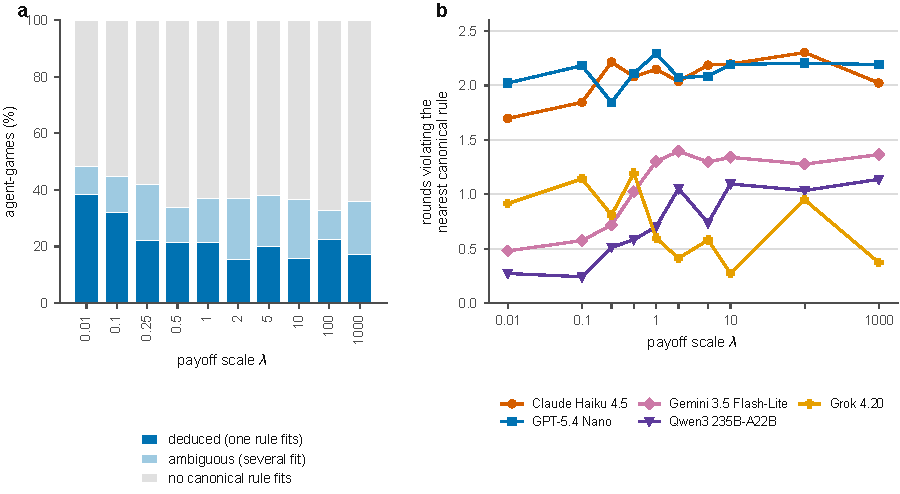
\includegraphics[width=\textwidth]{fig4_strategy.pdf}
\caption{\textbf{How closely play follows the canonical memory-one rules,
against the payoff scale.} Both panels are computed by exact matching, with no
learned component.
(a) Provenance of the strategy read-out, pooled over the five models; the
per-model trends, which do not all have the same sign, are in
table~\ref{tab:strategy}.
(b) Mean number of rounds, out of the ten played, violating the nearest
canonical rule.}
\label{fig:strategy}
\end{figure}

\begin{figure}[t]
\centering
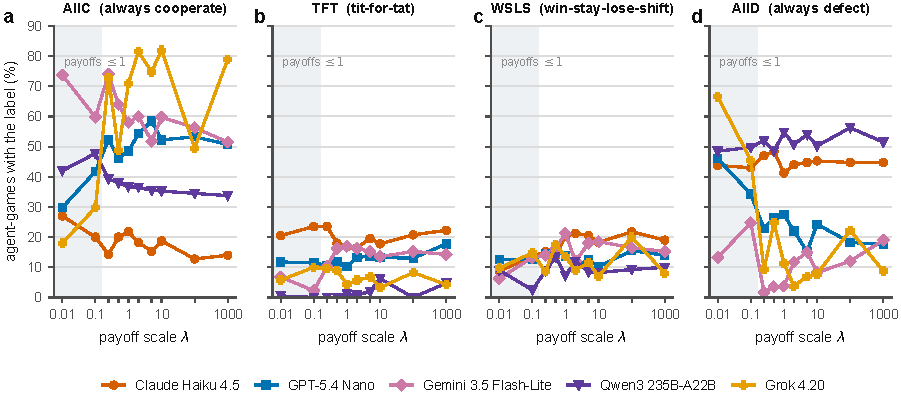
\includegraphics[width=\textwidth]{fig5_strategy_mix.pdf}
\caption{\textbf{Share of agent-games carrying each canonical label, against
the payoff scale.} One panel per canonical rule: (a) AllC, (b) Tit-for-Tat,
(c) Win-Stay-Lose-Shift, (d) AllD. Each point is the share of that model's 400
agent-games at that scale carrying the label, and shaded bands mark the two
scales at which every payoff printed is at most 1. The AllC and AllD panels rest
partly on exact rule matching, whereas the Tit-for-Tat and
Win-Stay-Lose-Shift labels are $94.6\%$ and $97.1\%$ attributions made where no
canonical rule fits, and should be read as a resemblance rather than as an
identification.}
\label{fig:mix}
\end{figure}

\subsection{The effect is present before any strategic interaction}

A rescaling could act through the course of play, by changing how a model reads
its opponent's history, or on the reading of the matrix itself. The opening move
separates the two: at round 1 nothing but the matrix and the instructions has
been seen.

The effect is already present at round 1 (figure~\ref{fig:firstmove}): in four
models of five the range of opening-move cooperation across the ten scales
exceeds the range over rounds 2 to 10, by factors of 2.0 in Claude Haiku 4.5,
1.9 in Gemini 3.5 Flash-Lite, 1.3 in GPT-5.4 Nano and 1.2 in Grok 4.20; the
exception is Qwen3 235B-A22B. The two windows rest on 400 and 3{,}600 decisions
per cell, so their ranges are not variance-matched and these ratios are
descriptive rather than tests.

The reading we take from this is deflationary about dynamics. Whatever the
payoff scale does, most of it is already done before the game has begun. That
is the timing an initial disposition read off the magnitudes of the matrix
would produce. It does not rule out a further effect on how history is weighed,
and this design does not separate the two.

\begin{figure}[t]
\centering
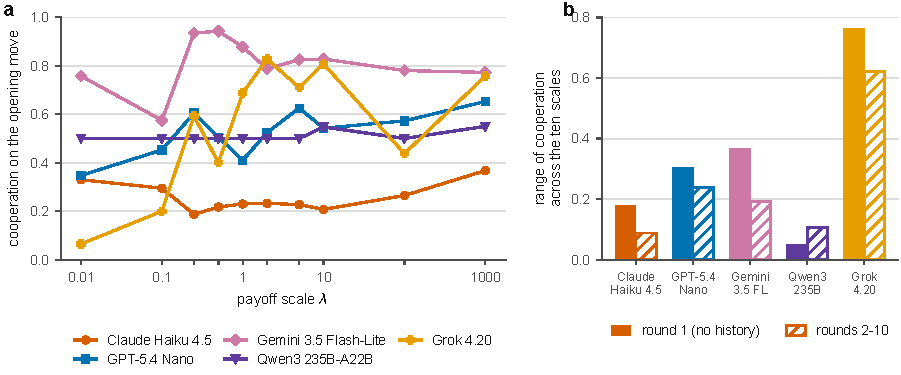
\includegraphics[width=\textwidth]{fig6_firstmove.pdf}
\caption{\textbf{Cooperation on the opening move, against the payoff scale.} At
round 1 the agent has seen only the matrix and the instructions.
(a) Cooperation on the opening move, one curve per model.
(b) Range of cooperation across the ten scales, on the opening move (solid) and
over rounds 2 to 10 (hatched).}
\label{fig:firstmove}
\end{figure}


% ---------------------------------------------------------------------------
% Section 4 (Discussion), Section 5 (Conclusion) and the Royal Society back
% matter, for paper_scaling/main.tex.
%
% Fragment only: paste after the Results section and before
%   \bibliographystyle{unsrtnat} / \bibliography{references}
%
% Numerals in this fragment, and nowhere else in it: 0.636 (Table 1, Grok 4.20
% cooperation range), 1.62 (the pooling attenuation), 1 (the sub-unit boundary)
% and 0.25 (a grid coordinate).  The corpus-wide provenance split (23.0 / 17.5
% / 59.6) previously lived ONLY in the Discussion; it has been removed here and
% must be stated in the strategy read-out subsection of Results instead.
% ---------------------------------------------------------------------------

\section{Discussion}
\label{sec:discussion}

\subsection{Payoff-scale invariance is violated}

The measurement reported here is unusual in having a null that is a theorem.
That property lets a movement in cooperation be read as a departure from an
invariance rather than as the difference between two conditions whose expected
gap was never specified. The predicted difference between a matrix and the same
matrix with larger cells is not small, or contested. It is zero.

All five models depart from it, and none is close to invariant. What makes the
departures hard to set aside is not their size but their structure: they are
present on the opening move, before any history exists, their size depends on
the language the game is posed in, they gate the persona instruction at a
boundary of magnitude, and they change what the transcripts look like as
sequences. Sampling variability alone is difficult to reconcile with a pattern
of that shape. The models appear to be responding to something in the matrix
other than the game it encodes, though this design does not identify what.

\subsection{Heterogeneity, and why pooled designs miss it}

The pooling result deserves emphasis, because it is the mechanism by which an
effect of this size could have gone unnoticed. The cause is arithmetic rather
than statistical: the shapes disagree, and several pairs are anticorrelated.
Heterogeneous effects that cancel are invisible to pooled designs by
construction.

In this panel the cancellation is partial rather than total. A main effect of
the payoff scale does survive the averaging, and it is significant, but it
carries a third of the variance its interaction with the model carries, and the
pooled range understates the typical model by a factor of 1.62: a statement
about an average model that nobody deploys.

A conclusion that changes when one model joins or leaves a panel is not a
conclusion about language models. The pooled estimate is therefore not a weaker
version of the per-model result but a different quantity, and it is not a
question of power either: more dyads or more models only tighten the interval
around an average of curves that point in different directions. The remedy is a
per-model analysis, not a larger sample.

The same logic runs one level deeper: the effect depends on the prompt language
as well as on the model, so a per-model number pooled over languages is the same
trick played on a smaller stage. The heterogeneity is not a nuisance to be
averaged away. It is the finding.

\subsection{Implications for behavioural benchmarking of language models}

A cooperation rate published for a language model is currently understood as a
property of the model. On this evidence it is a joint property of the model, the
units the matrix was written in, and the language the game was posed in. The
units are the awkward member of that list, because they are the one nobody is
asked to record: framings get described, personas get quoted, prompts get
reproduced in appendices, while the payoff scale is fixed once, silently, on the
authority of a theorem saying the choice is empty. Two laboratories running the
same protocol on the same model, with matrices differing by a constant factor,
could report cooperation rates differing by as much as 0.636.

We would suggest that a scale-sensitivity measurement accompany a published
cooperation rate, in the way an error bar does, and be measured per model,
most of all where such rates leave the benchmark and become the parameters of a
population model.

\subsection{Interpretation and possible mechanisms}

Two observations constrain what an explanation must account for. The boundary
gating the persona instruction appears to be one of magnitude rather than of
notation, a separation only as strong as the single scale that supports it
(\S\ref{sec:results}); and the payoff scale moves how closely play tracks any
canonical memory-one rule at all, and shifts the mix of labels with it. The
scale is not turning a single dial marked cooperativeness; it is changing the
shape of the trajectory.

Several accounts are consistent with both. The printed magnitudes may be read as
stakes, which is exactly what a rescaling does not change; numerals of different
magnitudes are tokenized differently, so a representation that changes with the
digit string could change what follows from it with no notion of stakes
involved; training text may associate large quantities with caution; and
sub-unit payoffs may fall outside the range in which payoff-like numbers are
ordinarily met.

We can order none of these. The design measures departures from an invariance;
it does not manipulate tokenization, vary notation at fixed magnitude beyond
the one contrast above, or move the framing that supplies the stakes. Nothing
here should be read as identifying a mechanism.

There is a constructive reading as well as a cautionary one. A programme is
under way to widen the utility function beyond the economic consequences of an
action, so that the language describing the action enters it directly, with
sentiment analysis proposed as the measurement and the replicator dynamics named
as the destination~\citep{capraro2024language}. Our result sits one level below
that programme rather than beside it. The evidence for language-based
preferences comes from manipulations that could legitimately have mattered,
since a label carries connotation, whereas a positive rescaling carries none and
is inert by theorem, and the behaviour still moves. A utility that mixes a
payoff with a score computed from language is no longer scale-free in the payoff
argument unless the two terms are rescaled together, so before such an object is
carried into an evolutionary dynamic its invariance class has to be stated. What
these data say is that at least one class of agents does not behave as though
the payoff argument were scale-free, and that anything built to describe them
will have to account for it.

\subsection{Limitations and future work}

This design does not identify the mechanism inside the model that produces the
departures it measures across a broad but finite grid. Six models cannot
support claims about model families or about parameter
count, and what generalizes here is that the shapes differ rather than what any
one of them is. The corpus is one game, one prompt template family and one
horizon, so whether the same curves appear in other dilemmas or in longer play
is untested.

A sixth model, Gemini 3.1 Flash-Lite, was run on the identical grid and is
reported in full in the electronic supplementary material rather than here,
because its identifier names an unpinned preview endpoint and what was served
under that name during collection cannot be recovered
(\S\ref{sec:methods}). Two consequences are worth stating rather than leaving to
be discovered. First, it is the only model of the six whose strategy trend is
positive, so the four-of-five statement in \S\ref{sec:results} reads, over the
whole corpus, as four models of six moving one way, one showing no trend and one
moving the other; the second form is the one the corpus supports. Second,
including it changes no conclusion here: the all-six pooled range, attenuation,
shape correlations and variance decomposition are in the electronic
supplementary material, \S S8, and every sign, significance and ordering in them
agrees with the five-model versions reported above.

The panel dependence of the pooled main effect is a limitation of this study as
much as an argument about others. Our own pooled estimate would have been a null
had one model been absent from the panel, and it is not a quantity we would
defend for its own sake.

One feature of the stimuli bounds the language comparison. Two of the five
templates state the payoffs as penalties while phrasing the goal as maximizing a
reward, and we reproduced rather than repaired them so that the corpus matches
the published protocol. Because that wording is fixed across the ten scales it
cannot generate a scale effect, and the within-language sensitivities stand; it
does mean that a difference in level between two languages is not attributable
to the language alone.

Our reference for calling a departure large is the sampling variability of these
data, a bootstrap over dyads and a permutation null, rather than an independent
repeat of the whole protocol. A measured test-retest floor, from
sweeps re-run under identical conditions, is the obvious next measurement.

The strategy read-out carries a further caveat, which is why its provenance is
reported wherever a label appears (\S\ref{sec:methods}). A strategy is a decision
rule and not a decision, so it is never observed directly, and even where the
resident rule is fixed by construction, separating the memory-one rules from
observed play has been shown to need a long run of
observations~\citep{kim2021win}. Our trajectories are ten rounds long. The claim that play
becomes less rule-governed rests on exact matching and no learned component.
The classifier was validated to $20\%$ execution noise, which is two rounds in
ten, and in two of the five models play sits about that far from the nearest
canonical rule on average, so the read-out is working at the edge of the range
it was validated on.
The compositional claim uses labels the classifier supplies wherever the rules
leave the answer open, is unevenly anchored across the four rules, and is the
weaker of the two. Any reading of it as evidence that these models implement
Tit-for-Tat would be unsupported by our data.

\section{Conclusion}
\label{sec:conclusion}

A positive rescaling of a payoff matrix is the rare manipulation whose
predicted effect is not merely small but exactly zero. Five frontier language
models were played across ten such rescalings, and every one of them moved. The
movement is not a uniform bias a calibration could absorb: its shape differs by
model and its size by prompt language, so most of it disappears from any
analysis that averages models, and what survives the averaging depends on which
models happen to be in the average. That is how a departure of this size can
sit inside a literature that has not reported it.

What follows is a question about design rather than a verdict on any model. A
cooperation rate measured on a language model is reported as though the matrix
behind it were an arbitrary and therefore harmless choice. It is arbitrary, and
it is not harmless. The same argument extends to every invariance the theory
supplies, from shifts of the payoffs to relabelling of the actions, and each is
an equally cheap test of whether an agent is playing the game it was shown.

% ---------------------------------------------------------------------------
% BACK MATTER
%
% Printed order, read off published Interface Focus articles, which agree:
%   Acknowledgements, Ethics, Data accessibility, Declaration of AI use,
%   Authors' contributions, Conflict of interest declaration, Funding.
% Acknowledgements comes FIRST, not last.  Do not reproduce the "Contributor
% Information" or "Associated Data" headings seen in PMC renderings; those are
% PMC artefacts, not Royal Society sections.
% Set as bold run-in paragraphs, which is how the journal prints them.  These
% are the only unnumbered run-in headings in the manuscript; the body uses
% numbered \section and \subsection.  Keeping the statements in the manuscript
% is correct even though the submission system now also collects them as form
% fields.
%
% AUTHORS: SIX blocks below are placeholders and must be completed before
% submission.  They are marked  % >>> FILL IN <<<
% Data accessibility additionally carries two bracketed placeholders, the
% Zenodo DOI and the licence.  Royal Society policy refuses "available on
% request" and requires data AND code public, with a DOI, AT SUBMISSION.
% ---------------------------------------------------------------------------

\paragraph{Acknowledgements.} We thank the providers of the model-inference
compute used to collect the corpus.
% >>> FILL IN <<<  Name the provider of the model-inference compute or credits,
% and any contributor below the authorship bar.  Interface Focus prints
% Acknowledgements FIRST in the back matter, ahead of Ethics.

\paragraph{Ethics.} This work did not require ethical approval from a human
subject or animal welfare committee.

\paragraph{Data accessibility.} Editors and reviewers can reach all three
components of this work now, at [review link]: the analysis pipeline that
produces every figure, table and quoted number, with the tidy tables it writes
and the scripts that draw the figures (\path{Analysis/scaling/}); the transcript
corpus of language-model games, held as per-game records of the decisions,
payoffs and conditions of every dyad (\path{Dataset/data_fairgame_frontier_llm/});
and the synthetic corpus that trains the strategy classifier, which contains no
language-model output (\path{Dataset/noise_dataset/}). Raw per-turn request and
reply text was not retained. The same three components will be deposited under
[licence to be named] in a public archive issuing a citable digital object
identifier, [archive DOI], which will be in place at publication. Supplementary
material is available online.
% >>> FILL IN <<<  [review link] is the GitHub or private "for review" URL that
% editors and reviewers use at first submission; [archive DOI] and the licence
% are filled in when the archive is deposited, which must be done by
% publication.  The corpus form of the last sentence carries a numbered
% reference, e.g. "Supplementary material is available online [64]."  Three
% reference-list entries are required and none exists yet:
%   (1) @misc for the archived analysis code (Zenodo DOI, tagged release),
%   (2) @misc for the transcript + synthetic corpora (Zenodo DOI, CC-BY-4.0),
%   (3) @misc for the electronic supplementary material.
% Add the three @misc entries to references.bib and cite them here at the same
% time: citing them before they exist would leave the build with undefined
% references.  Pattern:
%   @misc{code2026scaling, author = {...}, title = {...}, year = {2026},
%         publisher = {Zenodo}, doi = {10.5281/zenodo.XXXXXXX}}
% Royal Society policy requires data AND code to be reachable by editors and
% reviewers at first submission, and states that "available on request" is not
% acceptable; a GitHub or private "for review" link satisfies this now, and a
% permanent DOI archive is required only on publication.  Before submission:
% paste the review link.  Before publication: deposit the corpus and a tagged
% release of the code, add both DOIs to references.bib as @misc entries, cite
% them from this paragraph, and name the licence.
% Note also that raw per-turn transcripts (prompt, raw reply, seed) were not
% archived for these six models; only the aggregated CSVs exist.  Do not
% promise the raw turns here.

\paragraph{Declaration of AI use.} Language models are the object of study here:
the transcripts analysed were generated by the six models named in
\S\ref{sec:methods}, through a hosted model-serving platform. Separately, we
used a large-language-model coding assistant to help implement the analysis
pipeline and to assist with language editing. All analytical choices,
statistical specifications and interpretations are the authors', every number is
produced by the archived pipeline and checked against the data by an automated
verification script (\path{Analysis/scaling/s08_verify_paper.py}), and no text,
figure or result was generated by an AI system without author verification.
% >>> FILL IN <<<  Royal Society policy requires this declaration to be specific
% and accurate, and reserves the right to ask for the prompts and outputs.  Check
% the two sentences above against what was actually done, and name the assistant
% and the serving platform explicitly if the Methods do not.

\paragraph{Authors' contributions.} % >>> FILL IN <<<
% CRediT roles, lower case, semicolon-separated per author, initials with full
% stops.  Permitted roles: conceptualization; data curation; formal analysis;
% funding acquisition; investigation; methodology; project administration;
% resources; software; supervision; validation; visualization; writing -
% original draft; writing - review and editing.  The journal prints the last two
% with an em dash; house style here forbids em dashes, so they are written with
% a hyphen and the typesetter will normalize them.  Pattern:
%   A.B.: conceptualization, formal analysis, methodology, software, validation,
%   visualization, writing - original draft, writing - review and editing;
%   C.D.: conceptualization, funding acquisition, supervision, writing - review
%   and editing.
All authors gave final approval for publication and agreed to be held
accountable for the work performed therein.

\paragraph{Conflict of interest declaration.} T.A.H. is a Guest Editor of the
theme issue to which this article is submitted, and took no part in the
editorial handling or the peer review of this manuscript. The remaining authors
declare that they have no competing interests.
% >>> FILL IN <<<  Replace if any author has a competing interest to declare,
% including employment by or funding from a developer of any model studied here.

\paragraph{Funding.} No funding has been received for this article.
% >>> FILL IN <<<
% Required even when there is none.  Either:
%   This work was supported by [funder] [grant number] (A.B., C.D.).
% or:
%   No funding has been received for this article.
% A blank Funding section is a production query.


\bibliographystyle{unsrtnat}
\bibliography{references}

\end{document}
